\documentclass{article}
\usepackage{polski}
\usepackage[utf8]{inputenc} % by użyć polskich znaków w systemach Linux używamy kodowania "latin2", dla Windows "cp1250" 
\usepackage{floatflt,graphicx,textcomp}
\usepackage{hyperref}

\title{Zastosowanie aplikacji Wiki w przetwarzaniu zespołowym \\ Referat z przedmiotu \\ Przetwarzanie zespołowe i techniki negocjacji}
\author{Anna Jaworska, Piotr Orłowski}

\date{\today}

\begin{document}
\maketitle
\tableofcontents
\newpage

\section{Wstęp}

	Niniejszy referat ma na celu zarówno przybliżenie czytelnikowi samego mechanizmu Wiki, który często mylnie kojarzony jest wyłącznie z Wikipedią jak również, na co wskazuje sam tytuł, przedstawienie możliwości zastosowania go w pracy zespołowej.

	\subsection {W nurcie WEB 2.0}

	
		\textit{WEB 2.0 jest rewolucją biznesową w świecie komputerowym, spowodowaną ruchem w stronę Internetu jako platformy, oraz próbą zrozumienia reguł zwycięstwa na tej platformie.
		\begin{flushright}
			Tim O’Reilly
		\end{flushright}
		}
		WEB 2.0 to nurt w świecie Internetu, o którym od 2004 roku mówi się coraz częściej\footnote{Warto wspomnieć, że istnieje również pojęcie WEB 3.0, odnoszące się do Internetu zbudowanego wokół Sieci Semantycznej}. Nurt, którego głównym celem jest danie użytkownikowi www jak największej możliwości interakcji, integracji i personalizacji stron internetowych, tworząc jednocześnie wokół portali internetowych żywe społeczności internautów, które rozwijają, aktualizują i chronią te strony przed czynnikami szkodliwymi, jednocześnie pracując w jakimś celu - chociażby gromadzenia wiedzy czy też rozwijania jakichś projektów badawczych bądź technicznych.


		Obok przeróżnych Wiki do nurtu tego zaliczamy m.in. blogi oraz wszelkie portale pokroju Naszej Klasy, Grona, Facebooka, YouTube czy też MySpace, które dają użytkownikowi bardzo rozległe możliwości personalizacji i edycji tych serwisów. 


		Pod względem technicznym strony WEB 2.0:
		\begin{itemize}
    		\item używają nowych technologii, jak np. AJAX czy Ruby on Rails 
    		\item udostępniają interfejsy XML, które umożliwiają innym stronom i programom korzystanie z ich danych (np. przez RSS lub Atom)
		\end{itemize}


		Pod względem działania na społeczność internetową warto wspomnieć o:
		\begin{itemize}
    		\item tworzeniu społęczności różnorodnych użytkowników wokół WEB 2.0
			\item rozpowszechnianiu i stosowaniu licencji Wolnego Oprogramowania
			\item częstym stosowaniu folksonomii\footnote{Folksonomia - słowo to jest neologizmem określającym praktykę klasyfikacji i tagowania wiedzy w Internecie przez użytkowników m.in. portali społecznościowych, Wikipedii etc.}
		\end{itemize}


		Inną charakterystyczną cechą WEB 2.0 jest zwykle przyjemna dla oka szata graficzna, niekoniecznie rozbudowana, jednak z charakterystycznymi pastelowymi kolorami, zaokrągleniami i dużymi czcionkami.

	
		Budowane wokół stron WEB 2.0 społeczności mają charakterystyczną cechę: najczęściej tylko niewielka część tych społeczności uczestniczy w edycji i dodawaniu informacji do stron. W przypadku np. Wikipedii ok 4\%\footnote{Wg statystyk firmy Hitwise (badania z 2007 roku)} użytkowników kiedykolwiek dodało wpis do encyklopedii, natomiast w przypadku serwisu YouTube już tylko 0,16\% użytkowników kiedykolwiek dodało jakiś film do serwisu. 		



% Wiki jest przedstawicielem nurtu zwanego WEB 2.0
% - Co to jest WEB 2.0
% - dlaczego Wiki jest jego przedstawicielem?
% - WEB 3.0: i co dalej?

	%we are moving from passive readers to active participants.

%       The reality is, Wikipedia is quite different from organizational wiki sites
%both because of its primary use — encyclopedia — and the way its community
%is structured. I often say it’s the most extreme instance of wiki in existence
%because everyone can see its entire contents, anyone can contribute, and people
%can do so anonymously.
%                                                                     there are
%two types of wiki communities — the all-virtual versus the wiki that mirrors a
%physical community

%Back-office to Front-office str 95
	\subsubsection{Wiki a Wikipedia}
	Wiele osób kojarzy Wiki wyłącznie z Wikipedią. Poprzez to skojarzenie automatycznie widzą w niej mechanizm dostępny dla wszystkich, który wszyscy mogą edytować i czasem wręcz wandalizować. Jednocześnie wydaje się to być mechanizm nie zapewniający jakiejkolwiek wiarygodności danych w nim umieszczanych i dodatkowo mało bezpieczny. Prawdą jest, że Wikipedia (z uwagi na wykorzystywany w niej silnik MediaWiki) jest Wiki. Jednak sama Wiki absolutnie nie musi przypominać Wikipedii, gdyż jest to machina, którą można wykorzystać w zupełnie inny sposób, która wcale nie musi być dostępna dla każdego i która wcale nie musi być mało wiarygodna. Autorzy tego referatu mają nadzieję, jeżeli dotąd uważał, że Wiki to to samo co Wikipedia, zmieni zdanie po zapoznaniu się z treścią kolejnych rozdziałów.
	\subsection{Rys historyczny}

%The first wiki, WikiWikiweb (http://c2.com/cgi/wiki?WelcomeVisitors),
%was created in 1995 by Ward Cunningham to document and collaboratively
%update information on software design patterns. Since then, wiki has grown
%steadily into one of the most important tools in today’s enterprise, and has
%become a fixture in popular culture thanks to the rapid rise and increasing
%influence of Wikipedia. It’s commonly thought of today as a so-calledWeb 2.0
%tool because of its proximity to blogs and social networks, but this is primarily
%because its popularity and name recognition has taken off in tandem with the
%Web 2.0 phenomenon.
%Wiki is the Hawaiian word for quick. According to Cunningham, he chose
%the words Wiki Wiki, or Wiki (short version), to describe this new tool after
%remembering that a counter agent at Honolulu International Airport had
%directed him to take the Wiki Wiki bus to travel between airport terminals,
%and had explained that wiki is the word meaning ‘‘quick’’ in Hawaiian
%(Cunningham, 2005).According to Cunningham in 2005, ‘‘I wanted an unusual
%word to name what was an unusual technology. I was not trying to duplicate
%any existing medium, like mail, so I didn’t want a name like electronic mail
%(email) for my work.’’
	\textbf{Krótkie kalendarium}
	\begin{itemize}
		\item \textbf{1995 WikiWikiWeb}
		\item 1998 TWiki
		\item 1999 PHPWiki
		\item \textbf{2001 Wikipedia}
		\item 2001 JSPWiki
		\item 2002 MediaWiki
		\item 2004 Wikia, Confluence
	\end{itemize}
	\textbf{Początki}
	\newline
	Historia Wiki sięga początków 1995 roku, kiedy programista Ward Cunningham stworzył na stronie swojej firmy\footnote{c2.com - wtedy domena firmy informatycznej Cunningham \& Cunningham} prototypowe WikiWikiWeb - portal programistyczny złożony z modyfikowalnych stron www, który z założenia miał ułatwiać programistom edycję i dyskusję nad tworzonym kodem i oprogramowaniem. Wkrótce idea modyfikowalnego portalu internetowego została podchwycona przez innych programistów i zaczęły powstawać klony WikiWikiWeb. 
	

	\subsubsection{Co to znaczy Wiki?}
		Słowo ``wiki'' w języku hawajskim, oznacza szybko. ``Wiki wiki'' to także autobusy kursujące pomiędzy terminalami lotniska w Honolulu. Warh Cunningham początkowo chciał nazwać swoje Wiki QuickWeb, jednak po wizycie na Hawajach słowo ``wiki'' spodobalo mu się do tego stopnia, że nazwał je WikiWikiWeb.
	\subsubsection{Wikipedia}
	W styczniu 2001 roku uruchomiona została encyklopedia internetowa Wikipedia, jeszcze wtedy na silniku UseModWiki. Założona przez ekonomistę Jimmyego Walesa, znacząco upowszechniła nazwę Wiki w świecie, jednocześnie powodując, że bardzo wielu użytkowników utożsamia Wiki właśnie z Wikipedia i tylko na tej podstawie ocenia ten typ aplikacji.
	
	\subsubsection{Wiki po 2004 roku}
	W roku 2004 pojawiła się Wikia - portal internetowy, w którym każdy może założyć własną Wiki na dowolny temat pod warunkiem, że będą tam wyświetlane reklamy lub zostanie wniesiona stosowna opłata. W tym samym roku pojawił się Confluence, rozbudowana, komercyjna Wiki do zastosowań biznesowych. Od tamtych czasów popularność Wiki wzrosła znacznie - wiele firm stosuje ją do przechowywania wiedzy w firmie i rozwoju projektów natomiast własne encyklopedie internetowe posiada już prawie każdy popularniejszy serial animowany, film, gra komputerowa czy też klub piłkarski. 

% - skąd Cunningham wziął ten pomysł?
% - historyjka o autobusie...
% - jak to ewoluowało i jak zmieniało się podejście innych ludzi
% 

%	\subsection{Wiki jako CMS}
%              Because Wikipedia resides on the open Web, people assume
%that if they used a wiki for internal collaboration anyone could change the
%information on any page, even if their edits result in inaccurate or completely
%erroneous information. The reality is quite different when a wiki is used inside
%an organization, a

%                                          most organizations don’t really know
%what they know, and are poor at transmitting new ideas and new plans in a
%way that’s understandable. Organizations are mostly organized around their
%current goals. Some organizations have a part that tries to improve the process
%for attaining current goals. But very few organizations improve the process of
%figuring out what the goals should be
%   As I read this, I realized that it’s a brilliant argument for why the wiki can be
%a vital tool for organizations. Because it doesn’t define the terms of interaction
%and collaboration from the outset, and allows structure to be created, modified
%and removed as needed, the wiki quickly becomes a desirable tool because
%it ‘‘learns’’ how people work as they work, not after the fact. This means it
%captures more of the actual process, giving them an opportunity to regularly
%look at how they collaborate, even during a current project.

%   In the wiki of a private organization, this kind of vandalism or erroneous
%editing is extremely unlikely to happen because the wiki is being used within
%an already established social and organizational structure. The fact is people
%just don’t abuse tools that are important to their professional work.
			
%Wiki versus Intranet Powered
%by Content Management System  str 98
	
% przetłumaczyt=ć to co powyżej - bo w sumie Wiki zamienia się w takie gie bo pisać w tym strony da się...

\newpage
\section{Stosowane języki programowania}
Pierwsza Wiki, WikiWikiWeb, powstała na autorskim silniku napisanym w języku Pearl. Wkrótce po zaakceptowaniu przez programistów formy tego portalu zaczęły stopniowo pojawiać się jego kolejne klony pisane w różnych językach. Te popularniejsze wkrótce wyewoluowały w potężne silniki z własną społecznością, które do dzisiaj stopniowo się rozwijają. Śmiało można powiedzieć, że jeżeli dobrze poszukamy, to znajdziemy aplikację typu Wiki napisaną w języku, który najbardziej nam pasuje. 
	\subsection{PHP} 
%wymienić wiki z tym jezykiem, skrytykować że wersja jezyka jest stara
	PHP to chyba najpopularniejszy język tworzenia Wiki, o czym świadczy to, że na 25 najpopularniejszych\footnote{Na podstawie danych z serwisu www.wikimatrix.net. Z serwisu tego pochodzą również wszystkie podawane w tym rozdziale statystyki.} Wiki aż 13 chociaż częściowo napisano w tym języku. Już w 1998 roku, kiedy był on jeszcze bardzo mało znany, powstał klon WikiWikiWeb o nazwie PHPWiki. Warto wspomnieć, że zarówno MediaWiki, w którym tworzona jest Wikipedia, jak i dość popularne DokuWiki powstają w PHP. Pod jednym względem silniki w tym języku są nieustannie krytykowane: używają najczęściej starych, uważanych już za mało bezpieczne i przestarzałe wersji języka PHP - przykładowo najnowsza MediaWiki używa wersji 5.0 (z 2004 roku) i wymaga instalowania dodatkowych łatek zabezpieczającyh.  
	\subsection{Java}
	Jest to obecnie druga najpopularniejsza technologia tworzenia Wiki. Powstał w niej m.in. Confluence (rozbudowana, komercyjna Wiki do zastosowań korporacyjnych) oraz JSPWiki - otwarta, używana zarówno w zastosowaniach prywatnych jak również jako podstawa portali Internetowych Wiki, którą rozwijały m.in. Sun i Apache Software Foundation.
	\subsection{Perl}
	Trzeci język Wiki. Jak już wspomniano wcześniej, w nim powstała prototypowa WikiWikiWeb. Obecnie najpopulaniejszym silnikiem powstającym w tym języku TWiki, jeden z bardziej rozbudowanych i popularnych do zastosowań biznesowych, oraz Foswiki, jego niekomercyjna wersja.  
	\subsection{Inne}
	Na podstawie informacji zawartych na wikimatrix.net można śmiało stwierdzić, że istnieją Wiki prawie we wszystkich używanych językach programowania. Są w śród nich silniki popularne, jak np. MoinMoin napisany w Pythonie (używany między innymi jako silnik oficjalnych Wiki systemów Ubuntu, Debian oraz Mercuriala). Jest również wiele takich, które są napisane raczej w celu udowodnienia, że można w tym języku stworzyć taki mechanizm. Przykładowo instnieje Sputnik napisany w Lua, GeboGebo stworzony w Tdbengine, jednoosobowe TiddlyWiki w Javascripcie, w pełni funkcjonalna WikiSH napisana w Shellu czy chociażby Wiki Over DNS. Krążą plotki\footnote{Na podstawie informacji z serwisu www.esolang.org.}, że istnieje w pełni funkcjonalna wiki napisane w Brainf*cku. 	
% wspomnieć, że wiki można napisać nawet w Javascripcie....

\newpage
\section{Technologie pomocnicze}
	\subsection{Systemy kontroli wersji}
	% o tym, że większość Wiki z niego korzysta do przechowywania danych...
	Niektóre Wiki, np. TWiki, PHPWiki czy JSPWiki stosują lub mogą stosować systemy kontroli wersji do przechowywania danych. Często aplikacja typu Wiki w praktyce może działać również jako pewnego rodzaju ``subversion dla ubogich'' - wersjonując tworzone przy jej pomocy dokumenty..  
\subsection{LDAP}

Wprowadzenie Wiki w firmie wiąże się z umieszczeniem w nim kont dla pracowników. W przypadku większych firm byłoby to niewydajne. Dlatego dojrzałe Wiki umożliwiają migracje użytkowników z zewnętrznych baz. Wspomagane sa technologie takie jak LDAP, Active Directory itp. Synchronizacja z takim rozwiązaniem pozwala na zarządzanie użytkownikami kompletnie niezależne od aplikacji Wiki co może pozytwniej nastawić administratorów do wdrożenia Wiki,  

Większość Wiki posiada typy użytkowników z różnymi uprawnieniami oraz umożliwia grupowanie użytkowników. Przy integracji z LDAP grupy już istniejace zostają przeniesione do Wiki. Administratorowi pozostaje jedynie nadanie im odpowiednich praw dostępu.

	%SSO , poziomy dostępu, 
	\subsection{RSS}
	Jako technologia reprezentująca Web 2.0 Wiki często używa i udostępnia interfejsy XML, np. RSS i Atom. Dobrym przykładem jest tutaj Confluence, który potrafi zarówno użyć RSSów i danych Atom innych serwisów internetowych i automatycznie przetworzyć je oraz umieścić na wybranych stronach Wiki jak i udostępnia własne interfejsy XML.  
	%o tym, że Wiki stosują takie technologie jak RSS i Atom...
\newpage
\section{Przechowywanie danych}
	Wiki mogą korzystać z różnych systemów przechowywania danych. Często bardziej dojrzałe projekty potrafią korzystać z kilku różnych (nawet jednocześnie) i umożliwiają dodanie innych od standardowych dzięki zastosowaniu mechanizmu wtyczek. Niektóre zaś, tak jak TrikiWiki wymagają pisania własnych, dedykowanych konkretnemu systemowi w którym instalujemy Wiki, wtyczek. 
	\subsection{Pliki tekstowe}
	Stosowanym zarówno przez pierwszą Wiki jak i projekty nowsze, także te dojrzałe, metodą przechowywania danych są specjalnie skonstruowane pliki tekstowe. Zarówno TWiki, PHPWiki jak i JSPWiki udostępniają taki sposób przechowywania informacji, natomiast w MoinMoin i DokuWiki jest to zasadniczo jedyna opcja przechowywania danych. Sposób ten ma zarówno wady jak i zalety. Zaletą jest niewątpliwie to, że sam silnik do działania nie wymaga ani bazy danych ani żadnego dodatkowego systemu np bazodanowego - wystarczy, że zainstalujemy go na serwerze i spersonalizujemy a może on już w pełni spełniać swoje funkcje. Rozwiązanie to ma natomiast zasadniczą wadę - pliki te najczęściej nie zapewniają wydajności wyszukiwania nawet porównywalnej z bazami danych i innymi systemami przechowywania informacji. 
	\subsection{Bazy danych}
	Najpopularniejszym obecnie wśród dojrzałych Wiki mechanizmem do przechowywania danych są bazy danych. Najczęściej stosuje się te z otwartym kodem źródłowym, jak np. MySQL, PostgreSQL i SQLite - tych baz używają np. MediaWiki, TikiWiki, aczkolwiek niektóre silniki, m.in. komercyjny Confluence czy też XWiki, obsługują również Oracle DB lub DB2 czy MS SQL. Zaletą użycia bazy danych jest dużo większa wydajność tego sposobu składowania informacji. Wadą jest niewiątpliwie to, że instalacja i konfiguracja samej Wiki staje się przez zastosowanie tego mechanizmu trudniejsza.
	% DokuWiki nie ma nawet Subversion... dlaczego co i jak jest w tym dobre
	\subsection{System kontroli wersji}
	Alternatywnym sposobem przechowywania danych przez Wiki są systemy kontroli wersji, m.in. już nieco archaiczne RCS\footnote{Revision Control System, poprzednik CVS}, który może stosować m.in. TWiki czy PHPWiki, czy też CVS (MoniWiki, PHPWiki). Nie jest to sposób bardzo popularny, jedak warto o nim wspomnieć z uwagi na to, że Wiki gdy takiego systemu nie używa to i tak najczęściej w jakiś określony sposób wersjonuje dane, których używa.
\newpage
\section{Edycja danych}
	\subsection{WYSIWY(M)G}
		%TinyMCE
	Odkąd wiki stały się popularne wśród użytkowników nieobeznanych z metajęzykami, 
w większości z nich pojawiły się edytory WYSIWIG\footnote{What You See Is What You (Might) Get - czyli ``dostajesz to, co widzisz''}. Edycja stała się bardziej przyjazna użytkownikowi. Dobrym przykładem jest tutaj TinyMCE - mały edytor tekstowy, który pozwala w prosty, podobny do MS Word, sposób edytować dokumenty Wiki. Dodatkową zaletą jest to, że pozwala on importować dokumenty Worda z zachowaniem ustawionego w nim formatowania, co jest bardzo istotne, gdy użytkownicy pracują głównie w tym edytorze i chcą wklejać tekst z niego do Wiki. Dla przeciętnych użytkowników Wiki to znaczące udogodnienie.
%   As wikis have grown more popular and entered the mainstream, wiki
%vendors have added WYSIWYG (what you see is what you get) editors to
%make the editing experience look and feel more like the Microsoft Word-style
%interface many people are used to. The primary benefit of a WYSIWYG editor
%is that it can ease the transition when people first start using a wiki, but here’s
%the rub: if it’s the only editing tool people use, the WYSIWYG editor offers a
%much more limited editing experience and prevents people from making the
%leap necessary to fully understand the power of a wiki.

	\subsection{WYMIWYG}
	
WYMIWYG\footnote{What You Mean Is What You Get - czyli ``dostajesz to, co miałeś na myśli''} to inny sposób na wprowadzanie danych do Wiki. Wymaga od użytkownika poznania zestawu komend, które umożliwiają np. pogrubianie tekstu, ustawianie wypunktowań, odnośników i wielu innych ustawień tekstu. Tekst wprowadzony przez użytkownika jest odpowiednio interpretowany i dzięki temu w wersji ostatecznej na Wiki pojawia się on w formie sformatowanej w zamierzony przez użytkownika sposób. System ten jest stosowany przez wiele Wiki, m.in. MediaWiki - silnik Wikipedii, DokuWiki i wiele innych. Podejście takie ma zarówno wady i zalety. Do wad należy zaliczyć to, że należy się go nauczyć i niekoniecznie jest intuicyjny, szczególnie dla użytkowników początkujących. Do zalet natomiast to, że pozwala on ograniczyć objętość danych używanych przez Wiki, rosnącą gwałtownie w przypadku zastosowania zbyt rozbudowanego formatowania.

	\subsection{Edycja w programach zewnętrznych}

Wiki niekonieczne musi być edytowana poprzez przeglądarkę. Przykładowo artykuł w Wiki zintegrowanej z MS Sharepoint może być edytowany jako zwykły plik tekstowy. Wymagana jest wówczas znajomość składni Wiki. Ponadto twórcy Confluence postawili na integrację z pakietem biurowym i podjęli już pierwsze próby zastąpienia wbudowanego w edytora zwykłym procesorem testu zainstalowanym u użytkownika, np. MS Word. Taka integracja ma jednak wiele ograniczeń, ponieważ parsery przenoszące format z procesora tekstu na Wiki są niedoskonałe. Ponadto składnie Wiki nie wspierają wszystkich opcji procesorów tekstu. 



	\subsection{Nazywanie artykułów}

Wiki przewidują różne podejścia do zagadnienia nazywania artykułów. Generalnie można wyróżnić trzy podejścia:
\begin{itemize}
\item unikalne nazwy artykułów w całej Wiki - występuje głównie w Wiki mniej rozbudowanych, gdzie artykuły identyfikowane są w bazie danych dzięki ich nazwom
\item unikalne nazwy w ramach jednego działu/namespace - bardziej wygodne identyfikowanie artykułów poprzez powiązanie ich z lokalizacją
\item dowolne powtarzalne nazwy - podejście najbardziej elastyczna, gdzie aplikacja Wiki dla każdego artykułu generuje indywidualny identyfikator; pozwala to na tworzenie stałych adresów do artykułów (www.przyklad.pl/id=1234 zamiast www.przyklad.pl/Artykul) oraz umożliwia wprowadzenie mechanizmu automatycznych przekierowań - jeśli użytkownik odwoła się do adresu powiązanego z nazwą artykułu i jego lokalizacją zostanie on automatycznie przeniesiony do nowej lokalizacji danego artykułu. 
\end{itemize}

Poza adresami artykułu nazwy mają także wpływ na tworzenie linków wewnątrz Wiki. Takie linki zwykle wymagają podania tylko nazwy artykułu w Wiki, bez domeny, jak przy linkach zewnętrznych. Niektóre Wiki udostępniają możliwość nazywania artykułów z pomocą CamelCase. Jest to pomysł podobny do stosowanego w językach programowania - nazwa składająca się z wielu słów zapisywana jest bez spacji, początek nowego słowa sygnalizuje wielka litera. Przy takim podejściu Wiki zaczyna automatycznie tworzyć linki za słów zapisanych w formie CamelCase. Jednakże odchodzi się od tego rozwiązania, ponieważ wielu użytkowników uważa je za nieestetyczne oraz istnieją problemy, gdyż wszystkie skróty zapisywane wielkimi literami interpretowane są jako CamelCase, co jest zwykle niepożądane.



\newpage
\section{Sposoby organizacji informacji}	
	\subsection{Przestrzenie nazw}
	

	Niektóre Wiki, np. MediaWiki, organizują informacje w przestrzenie nazw. Jest to koncepcja zapożyczona z obiektowych języków programowania. Dane artykuł może należeć do kilku przestrzeni nazw. Na przykład \"Adam Mickiewicz\" moze być umieszczony w przestrzeni nazw \"pisarze\" oraz \"Polacy\". Artykuły dzięki temu można przeglądać poprzez kategorie.   
 
\subsection{Hierarchiczna organizacja informacji}
Większość nowych Wiki wspomaga hierachiczną organizację informacji. Strona glowna takiej Wiki zawiera przewaznie listę działów. W ramach jednego dzialu tworzona jest drzewiasta struktura artykułów.  

	Istnienie działów pozwala stworzyć w organizacji iluzje istnienia wielu Wiki. Każdy projekt lub komórka w firmie może mieć swój dział. W większości Wiki każdy z działów może wyglądać inaczej. To podejście pozwala wizualnie wyróżnić różne grupy korzystajace z Wiki i przekazać użytkownikom kontrolę nad ich działem.




\subsection{Tagi}

	Niektóre aplikacje Wiki pozwalają dodawać do artykułów tagi. Grupowanie artykułów za pomocą tagów pozwala    na alternatywną klasyfikacje informacji zawartych w Wiki. Artykuły umieszczone w różnych działach, a dotyczące podobnej tematyki (np. opis rozwiązań problemów z narzędziami programistycznymi), mogą dzięki tagom być   przeglądane  w jednym widoku, niezależnie od ich położenia.
Ponadto obecność tagów pozwala na poglądowe zapoznanie się z tematyką artykułów umieszczonych na Wiki.

       %                                                             Tagging
%has emerged as one of the most effective ways to organize information because
%the organization is the result of a collaborative process where people create
%tags as needed to describe content, and instead of putting content in folders
%which is restrictive because a file can only reside in one folder, multiple tags
%can be assigned to a document by multiple people, which ultimately results in
%a better categorization of its content.


	
	

\newpage
\section{Zastosowania w pracy zespołowej}
Mechanizm Wiki, odpowiednio użyty, może znacząco ułatwić pracę realizowaną zespołowo. W niniejszym rozdziale zostaną przedstawione podstawowe zastosowania oraz problemy, które Wiki pozwala rozwiązywać dużo łatwiej. 

	\subsection{Budowa portali}  

Wiki może stać się bazą do zbudowania portalu firmy. Jako, że większość Wiki można dostosować do własnych potrzeb dzięki pluginom (zmienić układ, kolorystykę), stają się one doskonałą bazą do zbudowania strony internetowej dostarczającej informacji o firmie. 
Ponadto mechanizm Wiki odciąża programistów tworzących taki portal od konieczności implementacji większości mechanizmów, takich jak zamieszczanie artykułów czy wiadomości od firmy.
Kolejnym plusem jest łatwość zarządzania użytkownikami - pracownikami, którzy będą umieszczać informacje na portalu.


	\subsection{Gromadzanie wiedzy}

		Wiki może posłużyć w organizacji jako uniwersalne narzędzie do gromadzenia wiedzy i wymiany doświadczeń miedzy pracownikami. Wiele firm korzysta z systemów zarządzania wiedzą (Knowledge Managment systems), jednak służą one głównie do gromadzenia faktów i ustaleń wewnętrznych. Mają zwykle formę bardzo formalną.

	Wiki jest narzędziem bardziej elastycznym. Może posłużyć jako wsparcie dla systemu KM. Dzięki Wiki ludzie mogą pracować nad projektami w sposób bardzo podobny do naturalnej komunikacji. Dokumentacja tworzona na Wiki staje się bogatszy, niż zwykłe dokumenty, przede wszystkim dzięki łatwości i szybkości edycji. Chcąc zmodyfikować jakiś dokument nie musimy szukać go na dysku, ściągać z repozytorium. Wystarczy wejść na stronę Wiki, skorzystać z mechanizmu wyszukiwania i zmienić pożądany fragment. Zmiana stanie się od razu widoczna dla innych użytkowników, nie trzeba wysłać innym zmienionego pliku. Taka szybka edycja bardzo przypomina zwyczajna interakcję między ludźmi, gdzie jedna osoba rozpoczyna jakiś pomysł, a kolejne rozbudowują go i zadają pytania na jego temat.

	Niektóre Wiki można zintegrować z systemami zarządzania błędami. Przykładem może być Confluence, który można zintegrować z innym produktem firmy Atlassian - JIRA - narzędziem do zgłaszania błędów. Po zamknięciu ticketu samo zagadnienie i sposób rozwiązania można szerzej opisać na Wiki w sposób prosty odwołując się do konkretnego ticketu. Ponadto w Confluence można wyświetlać różne podsumowania na temat błędów zgromadzonych w systemie JIRA. Takie zestawienie może posłużyć do tworzenia automatycznych raportów o stanie prac w projekcie.

	Jedna instalacja Wiki może stać się w organizacji uniwersalnym narzędziem do gromadzenia wiedzy. Można zawrzeć w Wiki zarówno informacje handlowe, księgowe jak i dokumentacje poszczególnych projektów. Zgromadzenie takich danych za pomocą jednego narzędzia może być dużym ułatwieniem dla nowych pracowników, którzy muszą poznać tylko jedno narzędzie, która ma "wszystko". 


		%Błędy w oprogramowanie - testowanie
		%Dokumentacja
		%Wiedza wewnętrzna organizacji
%                Unlike KM systems, wikis focus completely on letting people
%work together online the same way they’d work in person, and approach
%knowledge as the product of that organic, nonlinear human connection and
%collaboration. 

	\subsection{Integracja z innymi narzędziami}

	Większość komercyjnych Wiki pozwala na integracje z popularnymi narzędziami biurowymi. Możliwa jest także integracja w narzędziami typowo programistycznymi. Wśród przykładów takich połączeń warto wymienić:

\begin{itemize}
\item Confluence i Word - artykuły Wiki można pobrać za pomocą WebDAV i  edytować w MS Word; po użyciu zapisania zmiany automatycznie zostaną zapisane na Wiki
\item TracWiki - Wiki zintegrowana z Trac pozwala trzymać dane o postępie prac i dokumentacje w jednym miejscu; TracWiki zawiera gotowe mechanizmu pozwalające odwoływać się do konkretnych ticketów czy też wersji kodu 

\end{itemize} 



	\subsection{Mniej mejli}
	\begin{center}
		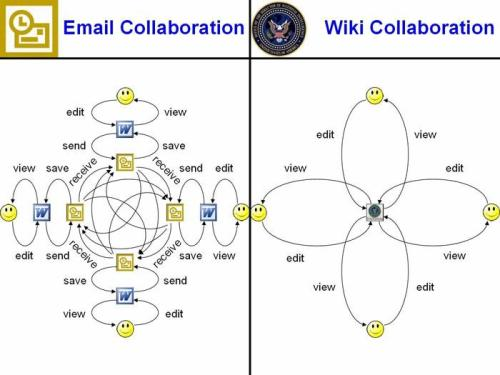
\includegraphics[width=11cm]{screenshots/wiki_collaboration2.jpg}
	\end{center}
		Ograniczenie liczby emaili wysyłanych w firmie jest najważniejszym i najbardziej pożądanym\footnote{zdaniem Stewarta Madera} efektem zastosowania Wiki w firmie. Wiki pozwala w prosty sposób organizować pracę grupową w tak, że zamiast tworzyć dokumenty lokalnie i wysyłać je sobie co jakiś czas wprowadzając zmiany, pracownicy mogą tworzyć je online i online zmieniać je, aktualizować, uściślać itp. bez konieczności oczekiwania na mejl od współpracownika. Czas zyskany w ten sposób pracownicy mogą poświęcić np. na rozwój samej Wiki, co jest działaniem zdecydowanie lepszym niż bezczynne czekanie.

		Wprawdzie istnieją inne, często bardziej rozbudowane mechanizmy wieloosobowej pracy nad dokumentami, jak chociażby SVN, google.docs\footnote{google.docs w przeciewienstwie do innych wymienionych daje nieco wątpliwy poziom bezpieczeństwa}, CVS i inne, to przy odpowiednio skonfigurowanej Wiki, z dobrze dobranymi szablonami, edytorami, otagowaniami i innymi udogodnieniami, jakie może ona dać, praca zespołowa przy użyciu tego typu aplikacji może być po prostu prostrza i bardziej dostępna dla przeciętnego użytkownika komputera.
%                             By reducing the number of general emails, people
%will be more likely to pay attention to the few that really do affect them, and
%by putting more specific communication on the wiki, people can identify and
%keep up with what’s most relevant to them.


%    eep in mind that I’ve just given the simplest example with only two
%people. If it can be this difficult for only two people to ‘‘collaborate’’ over
%email, imagine how these problems can balloon exponentially when more
%people are involved! A new wiki user recently told me a story of how it took
%three days to reconcile the edits that had gotten out of control when twelve
%people tried to use email to collaborate on a press release. The edits themselves
%didn’t take that long — within a few hours after the file had been emailed
%to everyone, twelve distinct files were returned with twelve different sets
%of edits!

	\subsection{Pisanie publikacji}

		Jednym z nietypowych zastosowań Wiki może być użycie jej do napisania artykułu naukowego lub książki. Takie formy publikacji zwykle wymagają pomocy korektora czy po prostu informowania wydawcy o postępie prac. Pisanie książki na Wiki pozwala wydawcy śledzić postęp prac autora, na bieżąco zgłaszać uwagi a nawet wprowadzać korektę. Przykładem książki napisanej w Wiki, jest wykorzystana  do stworzenia tego referatu książka Wikipaterrns\footnote{Wikipatterns, Stewart Mader, Wiley Publishing, Inc., 2008}.

	%ksiązki, artykuły
	%wydawaca/redaktor ma staly wglad w postepy prac

	\subsection{Wiki jako współdzielony dysk}
%str 99 beware of svn
		Przechowywanie plików na współdzielonych przestrzeniach dyskowych jest powszechnie praktykowane w wielu firmach. Projekty programistyczne są zwykle przechowywane w systemie wspomagającym kontrolę wersji, takim jak SVN. Sam kod to jednak nie jedyne dane przechowywane w firmie. 

		Przeciętne użytkownik komputera nie musi umieć posługiwać się SVN. Analityk czy też księgowy może niechętnie podejść do pomysłu przechowywania dokumentów w repozytorium, które może wydać się skomplikowane w użyciu i często brakuje dla niego prostego graficznego interfejsu. Ponadto repozytoria zapewniają wsparcie tylko dla plików tekstowych. 

		Wiki dzięki mechanizmowi załączników do artykułów może zostać zaadaptowana w firmie jak pewna forma współdzielonego dysku. Pliki można udostępniać dostarczając ich opis na stronie Wiki. Ponadto z istnienia niektórych z nich można wręcz zrezygnować - zwyczajne dokumenty tekstowe można przechowywać po prostu jako strony Wiki.

		Nie stworzy to problemu w przypadku konieczności wysyłania takich dokumentów np, do klienta. Wcale nie trzeba udostępniać wewnętrznej Wiki. Wiele aplikacji Wiki udostępnia mechanizmy eksportu dokumentów do PDF lub dokumentów Word.

	\subsection{Żywiolowa wymiana wiedzy i pomysłów}

%tego pragnie Pan Samolot najbardziej

%                                                               That’s what makes
%a wiki so special; it enables the natural patterns of interaction that previously
%could only happen in a physical meeting — fast-paced discussion, overlapping
%ideas, quick decisions on changes, quick error correction, introducing different
%viewpoints and collaboratively working to reach agreement — but it removes
 %                                                     Back-office to Front-office  57
%the need for everyone to be in the same place at the same time, and it documents
%the interaction better than a traditional meeting could.


		Sposób pracy z Wiki bardzo przypomina naturalną ludzką interakcję. Dzięki Wiki zachowania występujące zwykle na spotkaniu moga zostać przeniesione w środowisko wirtualne. Wiki pozwala na prowadzenie dyskusji, dzieki mechanizmom komentarzy. Ponadto wszelkie błędy mogą zostać szybko poprawione przez osobę, która je znalazła. Pomija sie dzieki temu koneicznośc wysylania e-maila do autora tekstu. Twórca tekstu nie traci jednak kontroli nad zmianami - może je sledzić dzieki mechanizmom RSS, lub po prostu dzięki historii zmian na stronie.

		Współpraca wirtualna na Wiki zwykle przypada do gustu zespołom, które nie pracują w tej samej lokalizacji. Wspólna edycja dokumentu na Wiki może zastapić konieczność podróży i spotkania. 

%	\subsection{Szybsza edycja} to powiela to co zostało napisane już wcześniej, więc tego nie pisze :P
%tego też pragnie Pan Samolot :)

%   By contrast, if we were using a wiki, you might see the wiki page at 2:55 P.M.
%waiting for your input, and decide to give it a quick read. If you get a great
%idea, want to make some minor changes, or even just notice a typo, all you
%have to do is click ‘‘Edit’’, make some quick changes, click ‘‘Save’’, and head
%off to your meeting. Now that the document has your input, collaboration
%can keep moving forward because I can revise based on your edits, send it to
%others for further input, and so on.

%Edycja stworzonego przez kogoś dokumentu Word może być kłopotliwa. Przykładowo, jesli 

\newpage
\section{Zanim wdrożysz}
Kiedy już zdecydujemy, że Wiki jest dokładnie tym mechanizmem, który chcemy zastosować np. w naszej firmie warto zastanowić się jeszcze nad kilkoma związanymi z tym oprogramowaniem problemami.
	\subsection{Problem licencjonowania}
	Zarówno przy wyborze Wiki komercyjnej jak i tej darmowej np. z otwartym kodem warto się zastanowić nad licencją, na której otrzymujemy to oprogramowanie.
	\subsubsection{Licencje komercyjne}
		Wiki komercyjne najczęściej sprzedawane są na określoną liczbę użytkowników. Warto jest to przemyśleć przed zakupem.  
	% - zastanowić się, które Wiki mają restrykcyjne ograniczenia, np. licencję IBM albo coś w ten deseń, o ograniczeniach na ilość użytkowników nie wspominając...
	\subsubsection{Licencje Wolnego Oprogramowania}
		W wypadku Wiki rozprowadzanych na wolnych licencjach warto dwa razy zastanowić się przed wybraniem silnika na licencji GPL. Licencja ta nakazuje upublicznianie wszelkich zmian w kodzie źródłowym a także kodu źródłowego, który wykorzystywany jest razem z kodem na tej licencji. W wypadku, gdy firma chciałaby stworzyć własną wtyczkę do takiego silnika, może ona nie być w ogóle zainteresowana ujawnianiem kodu z jakichś ważnych dla niej powodów. 
	% - wspomnieć o zagrożeniach związanych z licnejcją GPL
	% - wspomnieć o innych licencjach, np. tej M$ itp...
	\subsection{Sposoby instalacji}
		Najczęściej sama instalacja Wiki jest prosta i sprowadza się do któregoś z poniższych schematów:		
		\begin{description}
		    \item[``Cegła na enterze''] najprostrzy sposób sposób instalacji - sprowadza się ciągłego klikania dalej w kreatorze instalacji, ewentualnie zmieniając niektóre ustawienia na bardziej nam odpowiadające.
			\item[Menedżer pakietów] wiele popularnych otwartych Wiki udostępniono w repozytoriach różnych dystrybucji systemów typu linux, w związku z czym sama instalacja sprowadza się skorzystania z menedżera pakietów, np. yume lub aptitude.
			\item[make install] kiedy nie możemy skorzystać z menedżera pakietów należy pobrać ze strony domowej dystrybucję, w przypadku wersji linuxowej tarball, i postępować wg instrukcji do niej dołączonej. 
 		\end{description}


		Po zainstalowaniu Wiki przed rozpocząciem jej używania pozostaje skonfigurowanie jej do naszych potrzeb. Najczęściej wszelkie ustawienia zmieniamy przy pomocy odpowiedniej strony internetowej, którą udostępnia Wiki po instalacji. Warto zwrócić tu uwagę na:
		\begin{description}
			\item[Ustawienia lokalne] najczęściej musimy zacząć od ustawienia języka(języków), w którym dana Wiki będzie pisana, strefy czasowej i innych podobnych opcji charakterystycznych dla naszego rejonu geograficznego, kulturalnego itp.
			\item[Podłączenie bazy danych] w przypadku dystrybucji korzystających z bazy danych by móc dodawać cokolwiek do Wiki musimy wybrać odpowiednia bazę danych i skonfigurować połączenie z nią, ewentualnie załadować również wtyczkę, która umożliwi nam korzystanie z posiadanej przez nas bazy.
			\item[Inne] Do innych ustawień należy chociażby ustawienie emaila i hasła administratora systemu oraz skonfigurowanie użytkowników bądź zaimportowanie ich z np. LDAPa.
		\end{description}

	\subsection{Bezpieczeństwo}
	%kombinacje technologii z przkładami
		Wiki udostępniają zwykle odpowiednie mechanizmy uwierzytelniania użytkowników. Jeżeli udostępniamy naszą Wiki w Internecie warto pamiętać o zastosowaniu protokołu HTTPS zamiast nie zapewniającego żadnego bezpieczeństwa połaczenia i łatwego do podsłuchania HTTP
.
		Dodatkowo warto wspomnieć o tym, że bardziej zaawansowane silniki, szczególnie te komercyjne, często udostępniają również:
		\begin{itemize}
			\item poziomy dostępu użytkowników (ACL)
			\item mechanizm ról użytkowników (RBAC)
		\end{itemize}
	\subsection{Internacjonalizacja}
	%kombinacje technologii z przkładami
		Również wartym wspomnienia, a często zapominanym przez osoby instalujące Wiki zagadnieniem jest obsługa języków i internacjonalizacja. Jesto to szczególnie istotne, gdy firma, która chce uruchomić swoją Wiki posiada placówki w wielu krajach i istnieje szansa, że w przyszłości sama Wiki może zostać udostępniona pracownikom z zagranicy.

		
		Aby skutecznie zabezpieczyć się przed przyszłymi problemami warto na początku odpowiedzieć na 3 pytania:  
		\begin{itemize}
			\item Czy Wiki, której chcemu użyć obsługuje utf8?
			\item Czy posiada wszystkie wymagane wersje językowe?
			\item Czy baza danych i SVN danej Wiki też obsługują utf8?
		\end{itemize}
		Jeżeli odpowiedź na wszystkie te pytania jest pozytywna to najprawdopodobniej Wiki nie sprawi nam większych problemów w użytkowaniu pod względem internacjonalizacji.
	
	\subsection{Wsparcie techniczne}
		\subsubsection{Dla użytkowników indywidualnych}


			Z założenia użytkownik indywidualny nie ma dużych potrzeb z zakresu wsparcia technicznego. Nie opłaca mu się wykupywać, przeważnie drogiego, wsparcia przez telefon. Problemy z instalacją i obsługą Wiki taki użytkownik powinien rozwiązywać za pomocą różnych narzędzi dla społeczności, takich jak fora lub grupy dyskusyjne. Wybierając wiki dla użytkownika indywidualnego warto zwrócić uwagę na to czy te formy komunikacji między użytkownikami oprogramowania istnieją i czy ich użytkownicy są aktywni. Przydatna może się także okazać możliwość zgłaszania błędów twórcom oprogramowania.
		
		\subsubsection{Dla małych grup komercyjnych}


			Małe grupy to na przykład małe firmy lub grupy robocza w większych formach. Taki zespół powinien spróbować wybrać Wiki stworzoną w znanej sobie technologii, aby móc samodzielnie nią zarządzać. Istotne jest także, aby była to Wiki, którą można łatwo poszerzyć o kolejne sekcje czy działy, ponieważ bardzo możliwe (w przypadku grupy roboczej w większej firmie), że zachęceni sukcesem grupy znajdą się kolejni użytkownicy chętni do skorzystania z Wiki. 
	

			Kupowanie osobnego wsparcia, może okazać się zbędnym wydatkiem, jeśli pracownicy znają technologię w jakiej wykonana jest wybrana Wiki.
		
		\subsubsection{Dla dużych organizacji i firm}
		

			Duża firma powinna wybrać Wiki, która jest projektem dojrzałym. Ważne jest aby technologia użyta do jej wytworzenia była znana w firmie, co ułatwi pracę administratorom.

			Należy zwrócić uwagę na to, czy Wiki wspomaga technologie wspierające takie jak LDAP, co może przyspieszyć jej wdrażanie. Nie ma także sensu wdrażać Wiki korzystającej z bazy danych nie używanej w firmie. 

			Duża firma zwykle zmuszona jest poprzez regulacje wewnętrzne do zakupu wsparcia technicznego. Należy pamiętać o jego istnieniu i korzystać z niego bez wahania.

\newpage
\section{Wdrażanie}
%tego się nie dotykam - Piotrek
	\subsection{Problem zmiany polityki organizacji}


	W wielu organizacjach odpowiedzialnością za dokumenty z dokumentacją obciążane są konkretne osoby, nawet jeśli sam dokument tworzą zespoły. W takich przypadkach wdrożenie Wiki, która zakłada współpracę nad rozwojem dokumentów może zostać przyjęte z niechęcią. Osoby, które mają obawy związane z utratę kontroli nad kształtem dokumentu lub sądzącym, że ktoś ich pracę zniszczy, powinny zostać zapoznane bliżej z mechanizmami kontroli wersji dokumentów i przede wszystkim możliwością przywracania wcześniejszych wersji dokumentu. 

	Innym problemem może być niechęć dzielenia się pracowników wynikami swojej pracy. Mogą oni sądzić, że wykonana przez nich praca nie będzie doceniona, jeśli jej wyniki znajdą się na Wiki, zamiast w skrzynce mailowej szefa. Nic bardziej mylnego. Dzięki Wiki więcej osób może zapoznać się z wynikami pracy, a jej autor będzie znany, ponieważ umieszczane na Wiki wpisy mają wyróżnionego autora.

	Ponadto z punktu widzenia pracodawcy czas spędzony nad uzupełnianiem Wiki może być stracony. Nic bardziej mylnego. W przypadku zwolnienia pracownika jego wiedza pozostanie w firmie w postaci przyjaznych stron, z którymi z powodzeniem mogą zapoznać się jego następcy.

		

		


	\subsection{Zmiana sposobu obiegu dokumentów}


	W wielu organizacjach dokumenty podróżują głownie drogą mailową. Sprawia to, że pojawia się ich wiele wersji. Ponadto użytkownicy nie są pewni czy mogą dane dokument zmieniać po jego otrzymaniu. Do zmian zniechęca także konieczność ściągnięcia załącznika i  otwarcia go w innym programie, czy też nie posiadanie właściwego programu do jego otwarcia.

	Przykładem często pojawiającego się w organizacji dokumentu może być plan spotkania. Taki plan często pojawia na krótko przed samym spotkaniem. Jeśli zostanie wysłany np. 20 min przed spotkaniem, uczestnicy chcący zmienić lub skorygować niektóre jego punkty mogą nie zdążyć poinformować o tym organizatora, aby ten naniósł stosowane zmiany. Jeśli taki plan zostanie umieszczony na Wiki, każdy uczestnik będzie mógł bez problemu nanieść poprawki, bez ingerencji organizatora. Następnie taki plan może być użyty w trakcie samego spotkania - wyświetlony na rzutniku. Ponadto nic nie stoi na przeszkodzie, aby w trakcie trwania spotkania dopisywać na Wiki podjęte ustalenia na kolejne omawiane tematy.   
	
	\subsection{Problem własności informacji}

	W wielu złożonych z różnych działów organizacji zakłada się, że pracownicy jednego działu nie mają dostatecznej wiedzy aby pojąć czym dokładnie zajmuje się inny dział. To sprawia, że nie widzi się potrzeby udostępniania miedzy działami informacji o ich poczynaniach. 

	Ponadto w takich sytuacjach pojawia się brak zaufania do innych pracowników, aby powierzyć im wyniki swojej pracy, skoro ich ona nie dotyczy. Daje to osobie ukrywającej informacje pewne poczucie kontroli nad tym co dzieje się z posiadanymi przez nią dokumentami. Każdy, kto chce się czegokolwiek dowiedzieć o pracy takiej osoby, musi spytać ja osobiście. 

	Takie podejście obniża wydajność organizacji. Może zdarzyć się, że nagle zaczną być równocześnie realizowane bardzo podobne projekty, które można połączyć, ale ze względu na brak informacji nikt nie wpadnie na to odpowiednio wcześnie. Dochodzi również do redundancji dokumentów, wiele pracy wykonywanej jest jednocześnie przez wiele niezależnych osób.

	Z tych powodów należy zachęcać ludzi do dzielenia się na Wiki postępami i tematyką swojej pracy. Wiedza w dużej organizacji powinna być współdzielona, nawet jeśli potencjalnie nie zainteresuje innych pracowników. Przydatki, kiedy jednak okaże się przydatna mogą bardzo przyspieszyć niektóre działania. Ponadto, jeśli pracownik dokumentuje swoją pracę za pomocą ogólnodostępnego narzędzia, jego koledzy mogą mieć ogląd na to czym tak naprawdę zajmuje się ta osoba w danej organizacji. 

	\subsection{Change summary - Podsumowanie zmian i  jego przydatność w organizacji}
	
	Wiele Wiki udostępnia mechanizm podsumowania zmian. Zwykle ma on formę strony podsumowującej zmiany wprowadzone w Wiki przez pewien okres czas. Niektóre Wiki (np. Confluence) mogą także wysyłać takie raporty na e-mail. 

	Takie podsumowanie może przydać się kierownikom, aby ocenić jak Wiki przydaje się w organizacji. Zwykle są oni mile zaskakiwani aktywnością swoich pracowników. Ponadto edycje czy też komentarze na niektórych stronach mogą zwrócić uwagę kierownictwa na problemy obecnie występujące w ich firmie. 

	\subsection{Istotnośc pluginów}
	%wazne jest aby organizacja mogła sama rozszerzać soft wiki poprzez pluginy

	Niemal wszystkie Wiki budowane są w taki sposób, aby można było do nich napisać własne pluginy. Zwykle ich obecność w Wiki objawia się nowym poleceniem dostępnym poprzez składnię Wiki, lub rzadziej nową funkcjonalnością interfejsu. 

Możliwe jest przygotowanie pluginu pobierającego informacje poprzez usługę sieciową lub ze specyficznej bazy danych, innej niż ta przeznaczona dla Wiki. Ponadto można rozbudować funkcjonalność tak, aby wspierać charakterystyczne procesy firmy lub integrować się z aplikacjami dedykowanymi dla firmy. 

Takie możliwości pluginów mogą sprawić, że Wiki stanie się dla organizacji jeszcze bardziej uniwersalnym narzędziem. 

\subsection{Wikipatterns - reakcje ludzi na wdrożenie Wiki}

Doświadczenie wielu firm odnośnie wdrażania Wiki zostało zebrane w książce i na stronie Wikipatterns. \footnote{Wikipatterns, Stewart Mader, Wiley Publishing, Inc., 2008} Warto zwrócić uwagę na niektóre z tych wzorców zachowań.


\subsubsection{Spodziewana aktywność 90-9-1}

Wdrażając Wiki nie należy zakładać, że aktywność jej użytkowników będzie bardzo duża. Z doświadczeń firm korzystających w Wiki wynika, że ukształtuje się w następujący sposób: 
		\begin{itemize}
			\item 90\% czytających
			\item 9\% piszących od czasu do czasu
			\item 1\% maniaków
		\end{itemize}
Te proporcje użytkowników piszących do czytający można poprawić przygotowując przykłady i szablony artykułów, z których mogą skorzystać użytkownicy nie wiedzący od czego zacząć.

\subsubsection{Czempion}

Podczas wdrażania Wiki dla firmy zwykle pojawi się osoba będąca wielkim entuzjastą tego rozwiązania. Takiej osobie najlepiej powierzyć odpowiedzialność za rozwój Wiki. Głównymi jej zadaniami będą:
		\begin{itemize}
			\item pomaganie nowym użytkownikom w rozpoczęciu pracy z Wiki
		\item rozpowszechnianie idei Wiki, najlepiej w trakcie towarzyskich rozmów
		\end{itemize}

\subsubsection{Identyfikacja jest ważna}

Najczęściej pojawiająca się obawą przy wdrażaniu Wiki jest utrata kontroli nad tym, kto co napisał. Dlatego w Wiki firmowych najlepiej wyłączyć anonimową edycję.

Ponadto zaobserwowano, że użytkownik podpisujący się pod artykułem czy komentarzem własnym nazwiskiem zwykle chce pokazać się od najlepszej strony. Znacznie podnosi to jakość treści zamieszczanych na Wiki.


	\subsection{Historie wdrożeń} %jak w firmie/uczelni

\subsubsection{Sun Microsystems} %wikipatterns 61

	Firma Sun Microsystems udostępnia publicznie jedna z najlepszych Wiki o technologii. Do jej stworzenia został użyty Confluence. Każdy użytkownik internetu może zapoznać się z jej zawartością. Autorami artykułów są pracownicy firmy i eksperci zaproszeni przez nią do współpracy. Jest ich około 25 tys. Sprawia to, że poziom publikacji jest naprawdę wysoki.

	Ponadto Sun ma bardzo dobry regulamin Wiki, który jest bardzo zrozumiały. Można się na nim z powodzeniem wzorować tworząc regulamin firmowy. Jedną z bardzo pozytywnych cech jest system nagradzania aktywności uzytkowników za pomocą kolorowych gwiazdek. Nie wiążą się one z gratyfikacją pieniężną. Stają sie one bardzo miłą motywacją dla użytkowników.


\subsubsection{VMWare - konferencja VMWorld} %wikipatterns 61
		
Znana z oprogramowania do wirtualizacji firma VMWare co roku organizauje branżową konferencję. Firma postanowiła, że portal dotyczący konferencji zostanie zbudowany na podstawie wiki firmy Jivesoftware - Clearspace. Uczesnicy konferencji stali się uzytkownikami Wiki. Stworzono dodatkowy plugin do rejestrowania się na konferencje, który tak odciążył firmę, że oszacowała ona swoje zyski na 250 000\$.



\subsubsection{Disney}

Programiści z firmy Disney korzystają z TWiki do tworzenia dokumentacji gigantycznego między narodowoego portalu firmy. Zgodnie z ich raportami taka forma dokumentacji okazała się bardziej wydajna niż dotychczasowe tworzenie dokumentacji w wielu dokumentach.


\subsubsection{Texas Instruments}

Firma Texas Instruments wdrożyła TWiki w celu przchowywania w niej dokumentacji produkowanych urzadzeń. Pracownicy przygotowali wiele szablonów dokumentów, z ktorych korzystają na bieżąco. Co ciekawe kilki miesiący po wdrozeniu TWiki w firmie został przeprowadzony audyt ISO. Został on zakończony pełnym sukcesem. Pokazuje to, że Wiki nadaje się do przechowywania dokumentacji i wcale nie obniża standardu.

\subsubsection{Universitat Autonoma de Barcelona } 

Uniwersytet w Barcelonie wdrożył Wiki MoinMoin jako narzędzie elearning dla studentów.
Zadania dla studentów dostarczane sa na Wiki, Każda grupa studentów otrzymuje zadania i dział na Wiki, gdzie umieszcza dokumentację i postepy prac.

\newpage
\section{Podsumowanie}

Aplikacje Wiki już od blisko 15 lat pomagają w pracy zespołowej zarówno programistom jak i zwyczajnym pracownikom firm. Zasadniczą ich zaletą jest prostota edycji stron, co w połączeniu z możliwością stosowania mechanizmu szablonów, pozwala nawet mało zaawansowanym użytkownikom Wiki na dodawanie i edycję stron internetowych i dokumentów przy jej użyciu.

Wiki stało się na tyle powszechne, że czasem użytkownicy nawet nie są świadomi że używają aplikacji tego typu. Integracja Wiki z różnymi narzędziami wspomagającymi programistów staje się niemal standardem (Wiki dostępna jest w systemach typu Trac, eGroupware, Assembla). 

Na pewno nie jest to narzędzie doskonałe, jednak rekomendacja wielu firm i osób korzystających z różnych aplikacji Wiki w codziennej pracy zdecydowanie przemawia na plus tego typu oprogramowania.

Wiki jest stworzona z myślą przede wszystkim o pracy grupowej i w tej roli sprawdza się bardzo dobrze. Zadawala głównie prostotą i łatwością użycia.

Wiki można polecić każdemu - zespołowi znajomych pracujących nad wspólnym tekstem czy firmie tonącej w morzu dokumentów, druków i emaili. 


\newpage
\section{Dodatek - wykaz silników Wiki wspomnianych w tym referacie}
W dodatku tym w skrócony sposób opisano silniki Wiki wymienione w tym referacie.

\begin{description}
	\item[Confluence] rozbudowana, komercyjna Wiki stosowana np. przez średniej wiekości firmy i korporacje. Stworzona w technologii Java.  
	\item[DokuWiki] w pełni funkcjonalna Wiki nie potrzebująca bazy danych. Napisana w PHP. Posiada bardzo rozbudowany mechanizm wtyczek.
	\item[JSPWiki] jedna z pierwszych Wiki napisanych w technologii Java, dawniej m.in. silnik portalu firmy Sun, obecnie projekt rozwijany przez Apache Foundation. 
	\item[MediaWiki] jeden z najpopularniejszych silników Wiki. używa go między innymi Wikipedia. Stworzony w PHP.
	\item[MoinMoin] napisany w Pythonie, używany przez Wiki takich projektów jak Mercurial, Ubuntu, Debian i innych.
	\item[TiddleWiki] mała jednoosobowa Wiki napisana w Javascripcie i działająca raczej jako aplikacja PA (Personal Assistant).
	\item[Triki-Wiki] niemiecka Wiki napisana w PHP rozpowszechniana na licencji GPL. 
	\item[TWiki] komercyjna Wiki stworzona w Pearlu, dojrzała, z dużą ilością wtyczek. Jej niekomercyjną odmianą jest FosWiki.
	\item[UseModWiki] pierwszy silnik Wikipedii.
	\item[Wiki over DNS] eksperymentalna Wiki, która powstałą po to, by pokazać, że taką Wiki również można napisać.
	\item[WikiSH] w pełni funkcjonalna Wiki napisana w Shellu.
	\item[WikiWikiWeb] pierwsza Wiki, stworzona przez Warda Cunninghama w języku pearl. Jest działającym dotąd portalem programistycznym. 
	\item[XWiki] dojrzała Wiki napisana w Javie.
\end{description}


\newpage
\section{Bibliografia}
	\begin{itemize}
		\item 	Wikipatterns, Stewart Mader, Wiley Publishing, Inc., 2008
 		\item \url{http://www.oreillynet.com/pub/a/oreilly/tim/news/2005/09/30/what-is-web-20.html}
		\item \url{http://en.wikipedia.org/wiki/History_of_wikis}
		\item \url{http://www.wikimatrix.org}
		\item \url{http://en.wikipedia.org/wiki/Comparison_of_wiki_software}
		\item \url{http://www.esolang.org}
	\end{itemize}
\end{document}
